\documentclass[12pt,a4paper]{article}
\usepackage[utf8]{inputenc}
\usepackage{amsmath}
\usepackage{textcomp}

\usepackage{geometry}
\geometry{a4paper,left=25mm,right=25mm, top=2cm, bottom=2cm} 

\usepackage{verbatim}

 \usepackage{mathptmx}
 \usepackage[scaled=.90]{helvet}
 \usepackage{courier}

\usepackage[utf8]{inputenc}

\usepackage{listings}
\usepackage{color}

\usepackage{graphicx}
 
\definecolor{dkgreen}{rgb}{0,0.6,0}
\definecolor{gray}{rgb}{0.5,0.5,0.5}
\definecolor{mauve}{rgb}{0.58,0,0.82}

\pagestyle{empty}
\lstset{numbers=left,language=C++}
\lstset{showstringspaces=false,
basicstyle=\ttfamily\footnotesize,
breaklines=true,
tabsize=3,
commentstyle=\color{dkgreen},       % comment style
}

%keine einrückungen bei absatz
\parindent 0pt

\begin{document}
\title{Übung 1}
\author{Bernhard Selymes, Reinhard Penn}
\date{Oktober 2012}

\normalsize

%Pfad zu c++ Dateien
\newcommand{\CodePath}{../AdressManagement/AdressManagement/}

%Beginn des Dokuments
\section{Organisatorisches}

\subsection{Team}
	\begin {itemize} 
		\item Reinhard Penn, s1110306019 
		\item Bernhard Selymes, s1110306024
	\end {itemize}

\subsection{Aufteilung}
	\begin {itemize} 
		\item Reinhard Penn
			\begin {itemize}
				\item Planung
				\item Klassendiagramm
				\item Implementierung der Klassen Object, Roomlayout, Room, Side, Wall, Door
				\item Testen aller Klassen		
			\end {itemize}
		\item Bernhard Selymes
			\begin {itemize}
				\item Planung
				\item Klassendiagramm
				\item Implementierung der Klassen Object, Roomlayout, Room, Side, Wall, Door
				\item Dokumentation				
			\end {itemize}
	\end {itemize}


\subsection{Zeitaufwand}
	\begin {itemize}
		\item geschätzte Mh: 7h
		\item tatsächlich: Reinhard (10h), Bernhard  (10h)

	\end {itemize}


\section{Systemspezifikation}
Eine Software für einen Raumplan soll entwickelt werden. Ein Raumplan enthält mehrere Räume, jeder Raum hat 4 Seiten, die wiederum eine Wand oder ein Durchgang sein können. Die Räume sind alle gleich groß und liegen alle untereinander und nicht nebeneinander. Eine Wand hat eine Farbe, ein Durchgang ist offen oder geschlossen und verbindet einen oder zwei Räume - es gibt auch Durchgänge die nach draußen führen. Wenn zwei Durchgänge aufeinander treffen wird nur einer ausgegeben. Bei zwei Wänden werden beide ausgegeben. In der gesamten Datenstruktur können nur Objekte hinzugefügt, aber nicht gelöscht werden. Der gesamte Raumplan kann ausgedruckt werden. \\


\newpage
\section {Systementwurf}

\subsection {Klassendiagramm}

%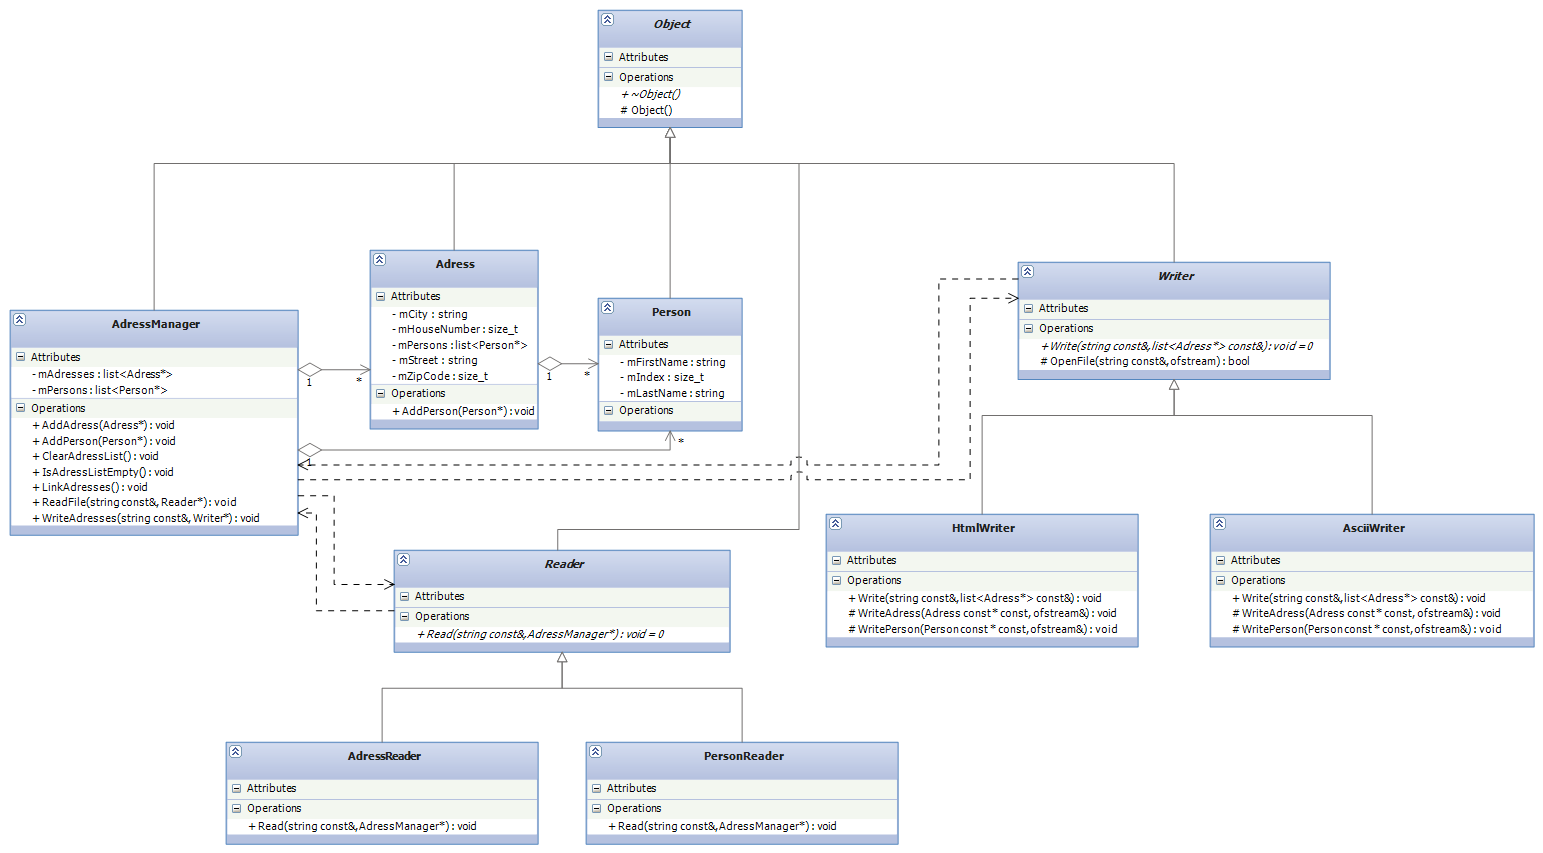
\includegraphics[angle=90,scale=0.7] {../Klassendiagramm.png}


\subsection {Komponentenübersicht}
\begin {itemize} 
	\item Klasse "Object":
	\newline
	Basis aller Basisklassen.
	\item Klasse "RoomLayout":
	\newline
	Beinhaltet die Räume und kann diese mithilfe einer Printfunktion ausgeben.
	\item Klasse "Room":
	\newline	
	Beinhaltet vier Seiten und kann mithilfe einer Printfunktion ausgegeben werden.
	\item Klasse "Side":
	\newline
	Abstrakte Klasse, von der Wall und Door abgeleitet werden. Speichert die Himmelsrichtung der Seite.
	\item Klasse "Wall":
	\newline
	Hat einen Member der die Farbe der Wand speichert.
	\item Klasse "Door": 
	\newline
	Speichert ob Door offen oder geschlossen ist und welche Räume von Door verbunden werden.
	\item Enumeration "Direction":
	\newline
	Hat vier Zustände: North, West, East, South

\end {itemize}

\newpage
\section {Komponentenentwurf}
\subsection {Klasse "Object"}
Abstrakte Basisklasse aller Klassen. Von ihr werden alle anderen Klassen abgeleitet. Beinhaltet einen virtuellen Destruktor.

\subsection {Klasse "RoomLayout"}
Besitzt eine Liste die Zeiger auf die Klasse Room beinhaltet, einen Zeiger, der auf den vorherigen Raum zeigt und einen Wahrheitswert, der angibt ob im letzten Raum im Süden ein Durchgang war. \\

\textbf {Methode "Print": } 
Gibt die Räume die in der Liste gespeichert sind der Reihe nach aus und merkt sich immer ob im vorherigen Raum eine Durchgang im Süden war. Wenn ein Durchgang war wird der Durchgang nur einmal ausgegeben. \\

\textbf {Methode "AddRoom":}
Fügt Räume zum Raumplan hinzu. Ein Raum wird nur dann hinzugefügt wenn die südliche Seite der vorherigen Raumes mit der nördlichen Seite des Raumes, der eingefügt werden soll, übereinstimmt oder der gesamte Raumplan noch leer ist. Wenn ein Durchgang war: Im vorherigen Raum wird bei Durchgang der aktuelle Raum hinzugefügt und beim Durchgang vom aktuellen Raum wird der vorherigen Raum gespeichert.
Weiters wird gespeichert ob der aktuelle Raum einen Durchgang im Süden hat und der Zeiger, der auf den vorherigen Raum gezeigt hat, zeigt jetzt auf den aktuellen Raum. \\

\subsection {Klasse "Room"}
Beinhaltet einen Vektor der Zeiger auf die Klasse Side hat.\\

\textbf {Methode "Print":} 
Gibt den Raum aus. Durchgang wird im Norden nicht ausgegeben, wenn im letzten Raum im Süden ein Durchgang war. Die restlichen Seiten werden ganz normal ausgegeben, eine Wand im Norden oder Süden wird durch 9 Sterne gekennzeichnet, im Westen oder Osten durch 5. Ein Durchgang wird durch ein "D" gekennzeichnet. \\

\textbf {Methode "AddSide":}
Fügt Seiten zu einem Raum hinzu. Eine Seite wird nur dann hinzugefügt, wenn noch keine Seite für diese Himmelsrichtung existiert. Der Vektor mit den Seiten wird nach dem Einfügen nach der Definiton der Enumeration sortiert: North, West, East, South. Wenn eine Seite ein Durchgang ist, wird im Durchgang der aktuelle Raum hinzugfügt. \\

\subsection {Klasse "Side"} 
Abstrakte Klasse, die eine Seite eines Raumes repräsentiert. Enthält einen Member der die "Direction" der Seite speichert und einen der angibt ob es ein Durchgang oder eine Wand ist. \\

\subsection {Klasse "Wall"} 
Repräsentiert eine Wand. Hat einen Konstruktor dem die Farbe und die Richtung der Wand übergeben werden. \\

\subsection {Klasse "Door"} 
Repräsentiert einen Durchgang. Hat einen Member der speichert ob die Tür offen oder geschlossen ist und einen Vektor der die Räume speichert, die der Durchgang verbindet. \\

\textbf {Methode "AddRoom":}
Fügt zum Durchgang einen Raum hinzu, wenn noch nicht die maximale Anzahl der Räume die ein Durchgang verbinden kann erreicht ist.

\subsection {Enumeration "Direction"}
\begin {itemize}
	\item North
	\item West
	\item East
	\item South
\end {itemize}

%
%\newpage
%\section {Source Code}
%
%\lstinputlisting[language=C++]{\CodePath Object.h}
%\newpage
%\lstinputlisting[language=C++]{\CodePath Object.cpp}
%
%\newpage
%\lstinputlisting[language=C++]{\CodePath RoomLayout.h}
%\newpage
%\lstinputlisting[language=C++]{\CodePath RoomLayout.cpp}
%
%\newpage
%\lstinputlisting[language=C++]{\CodePath Room.h}
%\newpage
%\lstinputlisting[language=C++]{\CodePath Room.cpp}
%
%\newpage
%\lstinputlisting[language=C++]{\CodePath Side.h}
%\newpage
%\lstinputlisting[language=C++]{\CodePath Side.cpp}
%
%\newpage
%\lstinputlisting[language=C++]{\CodePath Wall.h}
%\newpage
%\lstinputlisting[language=C++]{\CodePath Wall.cpp}
%
%\newpage
%\lstinputlisting[language=C++]{\CodePath Door.h}
%\newpage
%\lstinputlisting[language=C++]{\CodePath Door.cpp}
%
%\newpage
%\lstinputlisting[language=C++]{\CodePath Direction.h}
%
%\newpage
%\lstinputlisting[language=C++]{\CodePath main.cpp}


\newpage
\section {Testausgaben} 

\begin {verbatim}
Testcase0: Empty roomlayout


Testcase1: Roomlayout with empty rooms
Error occured in RoomLayout::AddRoom: Room is not full
Error occured in RoomLayout::AddRoom: Room is not full


Testcase2: Roomlayout with wrong rooms
*********
*       *
*       D
*       *
****D****


Testcase3: Roomlayout with correct rooms
*********
*       *
*       D
*       *
****D****
*       *
*       D
*       *
****D****


Testcase4: Roomlayout with correct rooms.
Trying to add a fifth side to one room
Error occured in Room::AddSide: Max amount of walls already reached
*********
*       *
*       D
*       *
*********
*********
*       *
*       D
*       *
****D****
\end {verbatim}


\end{document}